\documentclass{beamer}
\usepackage{amsmath, amsfonts}
\usepackage{listings}


\usepackage{amsmath, amsfonts}
\usepackage{listings}
\usepackage{xcolor}
\usepackage{graphicx}
\usepackage{booktabs}
\usepackage{tikz}
\usepackage{hyperref}
\usepackage{multicol}
\usepackage{lmodern}  
\usepackage{caption}
\usepackage{libertine}
\usepackage[libertine]{newtxmath}


\title[Enhanced Beamer Demo]{Graph Spectra and Hamiltonian Cycles }
\author{Szymon Wojtulewicz}
\date{\today}

\usetheme{default}

\usefonttheme{professionalfonts}


\definecolor{accent}{RGB}{130,160,255}
\definecolor{blockbg}{RGB}{240,240,245}
\definecolor{blockborder}{RGB}{220,220,220}

\setbeamertemplate{navigation symbols}{}
\setbeamertemplate{footline}[frame number]
\setbeamertemplate{blocks}[default]


\setbeamercolor{block title}{fg=black,bg=blockbg}
\setbeamercolor{block body}{bg=blockbg}
% \setbeamerfont{block title}{series=\sffamily\bfseries}

\definecolor{codebg}{RGB}{250,250,250}
\definecolor{keywordcolor}{RGB}{70,110,200}
\definecolor{stringcolor}{RGB}{200,130,130}
\definecolor{commentcolor}{RGB}{140,180,140}

\lstset{
  backgroundcolor=\color{codebg},
  basicstyle=\ttfamily\footnotesize,
  keywordstyle=\color{keywordcolor}\bfseries,
  stringstyle=\color{stringcolor},
  commentstyle=\color{commentcolor}\itshape,
  frame=single,
  breaklines=true,
  showstringspaces=false,
  tabsize=2
}


\begin{document}

\begin{frame}{Incidence matrix for the same graph}
  \begin{block}{}
    For a simple undirected graph \(G=(V,E)\) with vertex indices \(1,\dots,n\) and edges indexed \(1,\dots,m\),
    the (undirected) incidence matrix \(B_G\in\{0,1\}^{n\times m}\) has entries
    \[
      (B_G)_{v,e}=\begin{cases}
        1 & \text{if vertex }v\text{ is incident to edge }e,\\[4pt]
        0 & \text{otherwise}.
      \end{cases}
    \]
    (Each column has exactly two ones for a simple edge connecting two distinct vertices.)
  \end{block}
  \begin{columns}[T,onlytextwidth]
    \begin{column}{0.55\textwidth}
      \centering
      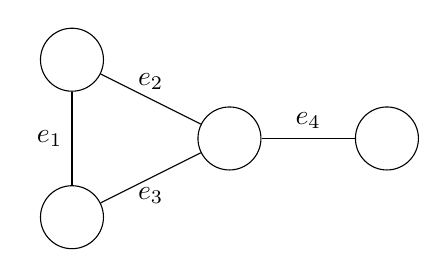
\begin{tikzpicture}[scale=1,auto,main node/.style={circle,draw,inner sep=1pt,minimum size=8mm}]
        \node[main node] (1) at (0,2) {};
        \node[main node] (2) at (0,0) {};
        \node[main node] (3) at (2,1) {};
        \node[main node] (4) at (4,1) {};
        \path
          (1) edge node[left]  {$e_1$} (2)
          (1) edge node[above] {$e_2$} (3)
          (2) edge node[below] {$e_3$} (3)
          (3) edge node[above] {$e_4$} (4);
      \end{tikzpicture}
    \end{column}
    \begin{column}{0.45\textwidth}
      \[
      B_G=\begin{bmatrix}
      1 & 1 & 0 & 0\\
      1 & 0 & 1 & 0\\
      0 & 1 & 1 & 1\\
      0 & 0 & 0 & 1
      \end{bmatrix}
      \]

      % \medskip

      Incidence matrix \(B_G\) for edges ordered
      $(e_1, e_2, e_3, e_4)$.
    \end{column}
  \end{columns}
\end{frame}


\end{document}
